\section{SOFTWARE ARCHITECTURE}
\subsection{System architecture layers}
The application consists of three layers:
\begin{itemize}
	\item \textbf{Presentation Layer}: contains the components that implement and display the user interface and manage user interaction.
	\item \textbf{Business Logic Layer}: is used as an intermediary for data exchange between the presentation layer and the data access layer. Business entities, or business objects, encapsulate the business logic and data necessary to represent real world elements. The business layer's goal is to minimize the complexity by separating tasks into different areas of concern.  
	\item \textbf{Data Access Layer}: includes methods which can interact with the database. When methods are called, it will connect to the database by using query and will return the corresponding results.  
\end{itemize} 
\begin{figure}[H]
	\centering
	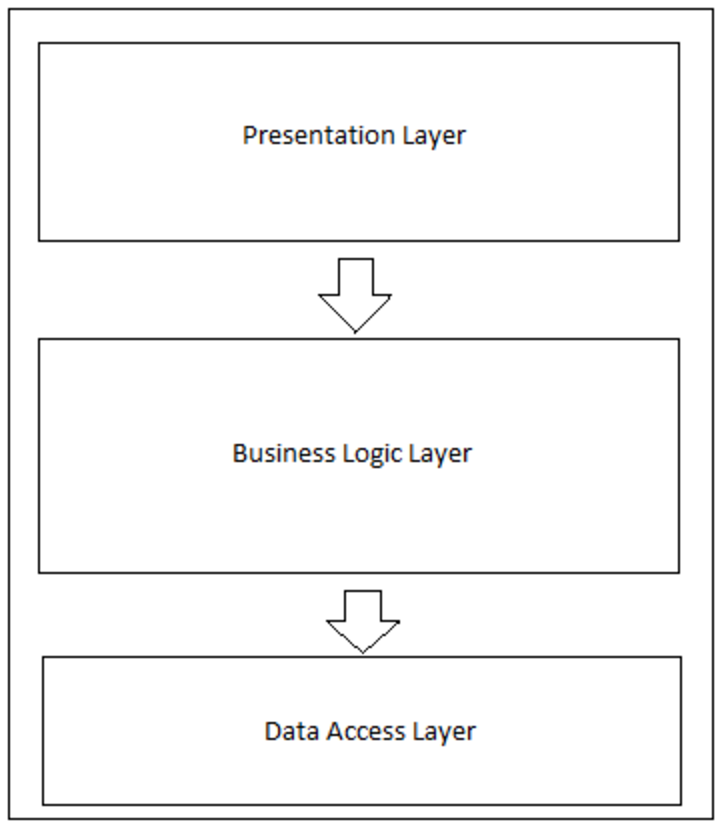
\includegraphics{Three_layered_architecture}
	\caption{Three-layered architecture}
\end{figure}
With a three-layered architecture, improving the modularity of the application will be simple and this can make it easier for developers to extend features in the future. Distinguishing among the different layers allows the development team to program according to the interfaces, thus allowing an easier distribution of the work.  
\subsection{Technologies used}
\begin{itemize}
	\item \textbf{Back-end and database}: JavaScript will be used to build the back-end of the application and the database will be based on Json files stored in Firebase.
	\item \textbf{Front-end}: the application will use HTML, CSS and Bootstrap for front-end.
\end{itemize}
\begin{figure}[H]
	\centering
	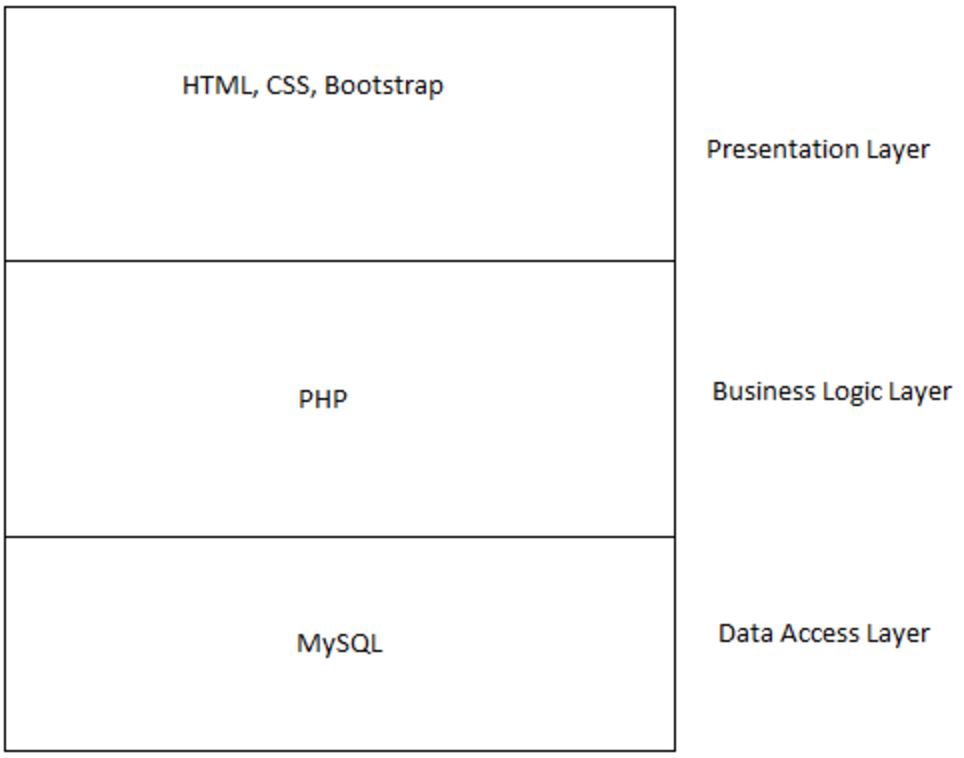
\includegraphics[width=14cm]{Technologies}
	\caption{The technologies in the three-layered architecture of the application}
\end{figure}